\chapter{Feature Masking for Object-Centric and Predictive Visual Representation}
\label{chap:feature_masking}
\section{Motivation}
Reflective guitar finishes and metal hardware generate highlights that can move with illumination and camera pose. A conventional RGB encoder may attend to these correlations rather than the target surface, tool contact region, defect, or protected obstacle. Background clutter and robot-body pixels can also dominate the learned representation. This chapter proposes a mask-guided extension of the force-aware IL framework. The design is preliminary and is presented as a research plan rather than a completed method.

\begin{figure}[t]
    \centering
    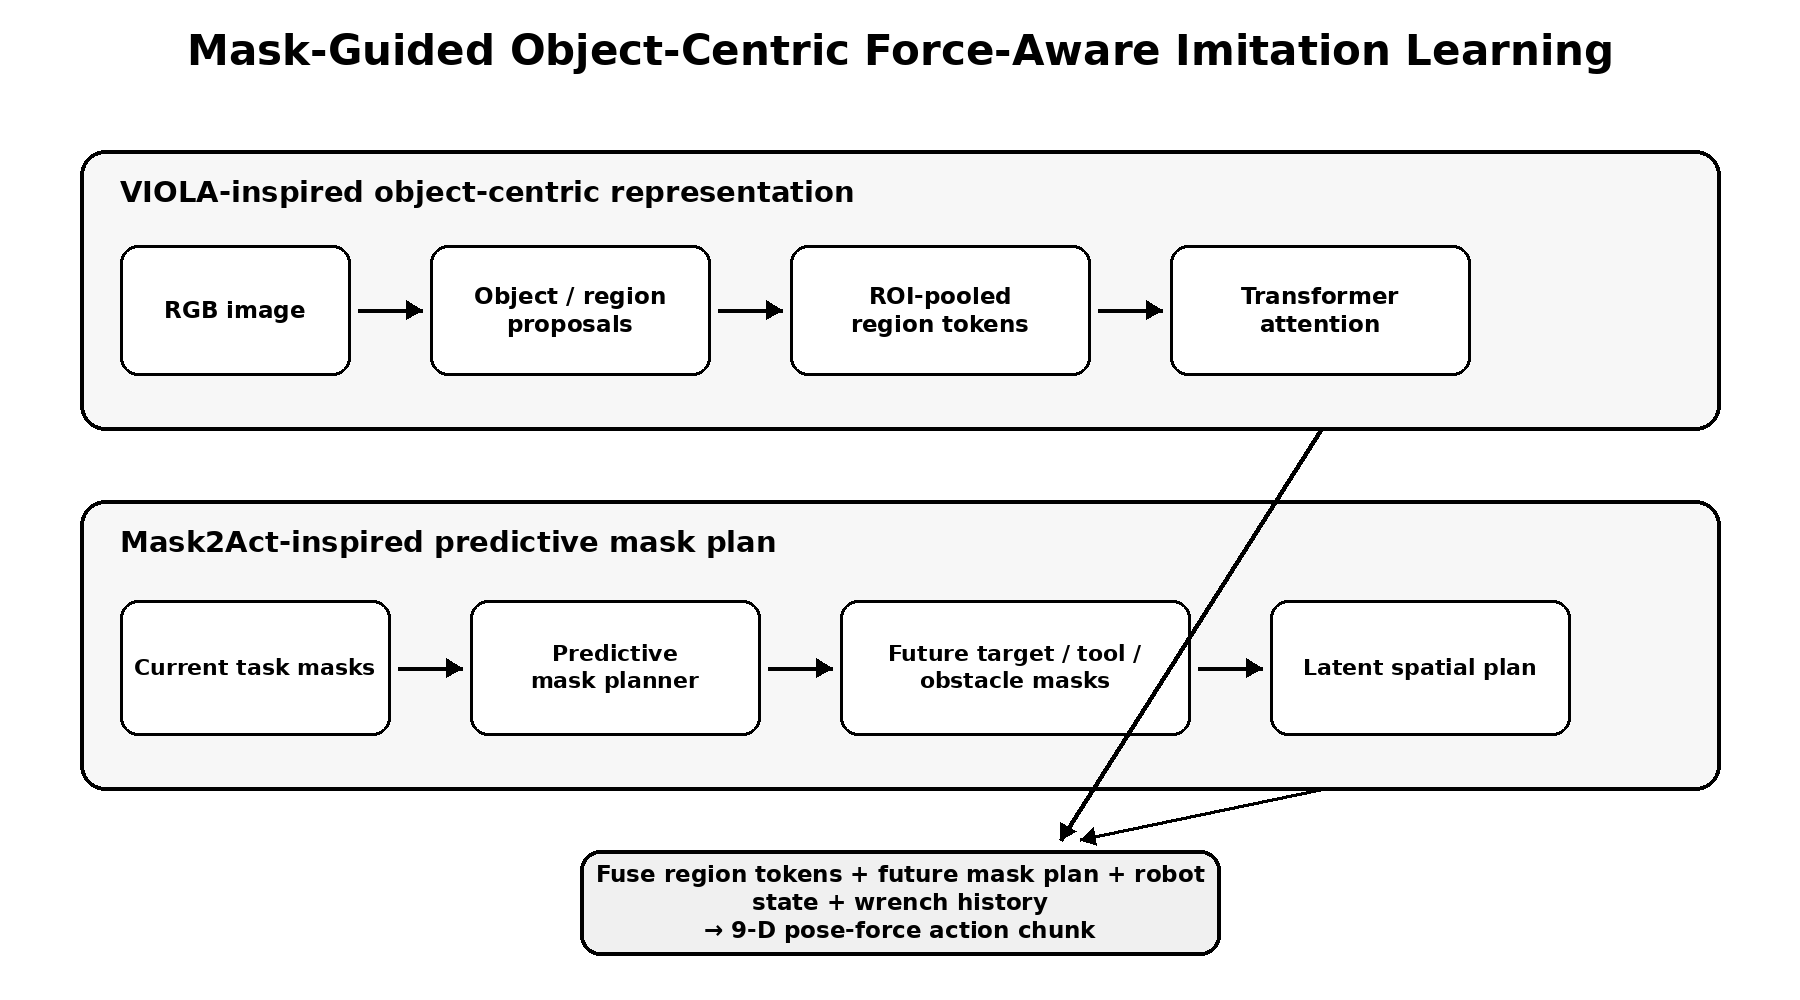
\includegraphics[width=0.98\textwidth]{./6.FeatureMasking/figs/feature_masking_architecture.png}
    \caption{Proposed integration of VIOLA-inspired object-centric region tokens and Mask2Act-inspired predictive mask plans with the force-aware IL policy.}
    \label{fig:feature_masking}
\end{figure}

\section{Task-Relevant Mask Definitions}
The proposed system represents four semantic mask types:
\begin{enumerate}
    \item \textbf{Target-processing mask} $M^{\mathrm{tar}}$: the region that should be polished;
    \item \textbf{Tool-footprint or contact mask} $M^{\mathrm{tool}}$: the visible or predicted contact footprint;
    \item \textbf{Protected-object mask} $M^{\mathrm{obs}}$: hardware, string anchors, fretboard, or other regions that must not be contacted;
    \item \textbf{Defect or condition mask} $M^{\mathrm{def}}$: scratch, haze, oxidation, stain, or local loss of gloss when such a region is visually detectable.
\end{enumerate}
Masks can be obtained from manual labels, a task-specific segmentation model, or a pretrained segmentation foundation model followed by temporal refinement. The thesis should distinguish mask-generation error from policy error.

\section{VIOLA-Inspired Object-Centric Region Tokens}
VIOLA uses object proposals from a pretrained vision model to construct object-centric representations and a transformer policy to attend to task-relevant visual factors~\cite{zhu2023viola}. The proposed polishing adaptation replaces generic household-object proposals with region proposals relevant to contact: target surface, tool footprint, protected hardware, and defect region.

Given image feature map $\mathbf{Z}_t$, each proposal or mask $M_t^i$ produces a region token through ROI pooling or masked average pooling:
\begin{equation}
\mathbf{r}_t^i = \mathrm{Pool}(\mathbf{Z}_t,M_t^i).
\end{equation}
The set of tokens $\{\mathbf{r}_t^i\}$, a global image token, robot-state tokens, and wrench-history tokens are processed by a transformer. Attention weights provide an interpretable indication of which region contributes to the pose--force prediction, although attention alone should not be treated as proof of causal relevance.

\section{Mask2Act-Inspired Predictive Mask Plans}
Mask2Act learns a planner from action-free video by predicting future masks of task-relevant objects and uses the latent plan to guide an executor trained with robot action data~\cite{zhang2025mask2act}. For polishing, the proposed planner predicts a sequence of future target, tool, and protected-object masks:
\begin{equation}
\hat{\mathbf{M}}_{t+1:t+H}=\mathcal{P}(I_{t-h:t},\mathbf{M}_{t-h:t},g),
\end{equation}
where $g$ specifies the local task or target region. The predicted future masks encode how the contact footprint should move over the target while remaining separated from protected hardware. Unlike future RGB prediction, the mask sequence suppresses texture and illumination details that are unrelated to motion.

The action executor conditions on the future mask plan, robot state, and wrench history:
\begin{equation}
\mathbf{A}_t=\mathcal{E}(I_t,\hat{\mathbf{M}}_{t+1:t+H},\mathbf{s}_t,\mathbf{H}_t^w).
\end{equation}
The future mask sequence is a latent spatial plan, not a substitute for force sensing. It specifies where the task-relevant regions should move in image space, while the wrench history informs whether the physical contact is correct.

\section{Combined Mask-Guided Force Policy}
The full proposed architecture contains two complementary branches. The VIOLA-inspired branch provides object-centric region tokens at the current time. The Mask2Act-inspired branch predicts future masks as a high-level spatial plan. These representations are fused with robot state and force history before the flow-matching action generator.

The policy can be trained with a combined objective:
\begin{equation}
\mathcal{L}=\mathcal{L}_{\mathrm{action}}+\lambda_{\mathrm{mask}}\mathcal{L}_{\mathrm{future\ mask}}+\lambda_{\mathrm{cons}}\mathcal{L}_{\mathrm{contact\ consistency}},
\end{equation}
where $\mathcal{L}_{\mathrm{action}}$ is the behavior-cloning or flow-matching loss, $\mathcal{L}_{\mathrm{future\ mask}}$ supervises future masks, and $\mathcal{L}_{\mathrm{contact\ consistency}}$ encourages agreement between predicted tool masks and measured contact phases. The exact consistency term remains to be finalized.

\section{Training Strategy}
A staged training procedure is proposed:
\begin{enumerate}
    \item train or adapt the mask extractor on target, tool, hardware, and defect annotations;
    \item pretrain the future-mask planner from action-free or demonstration videos;
    \item train the force-aware executor using robot demonstrations while freezing or slowly fine-tuning the planner;
    \item jointly fine-tune the combined policy with conservative learning rates and validation on unseen lighting and background conditions.
\end{enumerate}
Action-free video is particularly attractive because local polishing demonstrations with synchronized robot action and force are expensive. However, human and robot tool morphology differ, so the predicted mask plan should focus on target and contact-footprint motion rather than exact human hand motion.

\section{Planned Ablations}
The feature-masking study compares:
\begin{enumerate}
    \item raw RGB baseline;
    \item RGB multiplied by a binary target mask;
    \item RGB plus mask as an additional channel;
    \item VIOLA-inspired object-centric region tokens;
    \item Mask2Act-inspired future-mask latent plan;
    \item combined region-token and future-mask model;
    \item each of the above with and without wrench history.
\end{enumerate}
Evaluation includes task success, local coverage, collision, force metrics, generalization to lighting and background changes, sensitivity to mask noise, and representation analysis using occlusion tests and controlled perturbations. The combined model should be accepted only if the benefit exceeds the added segmentation and training complexity.
